\section{Einführung und Überblick}

\begin{definition}{Software Engineering}
Software Engineering ist eine systematische und strukturierte Entwicklung von Software:
\end{definition}

\begin{corollary}{Kernprozesse}

\begin{minipage}[t]{0.6\textwidth}
\begin{itemize}
  \item Anforderungserhebung
  \item Systemdesign/technische Konzeption
  \item Implementierung
  \item Softwaretest
  \item Softwareeinführung
  \item Wartung/Pflege
\end{itemize}
\end{minipage}
\begin{minipage}[t]{0.38\textwidth}
\textbf{\textcolor{frog}{Unterstützungsprozesse}}
\begin{itemize}
  \item Projektmanagement
  \item Qualitätsmanagement
  \item Risikomanagement
\end{itemize}
\end{minipage}
\end{corollary}


\begin{concept}{Dimensionen der Softwareentwicklung}
\begin{itemize}
    \item Requirements (Bekannt - Unbekannt)
    \item Technology (Bekannt - Unbekannt)  
    \item Skills/Experience (Vorhanden - Nicht vorhanden)
\end{itemize}
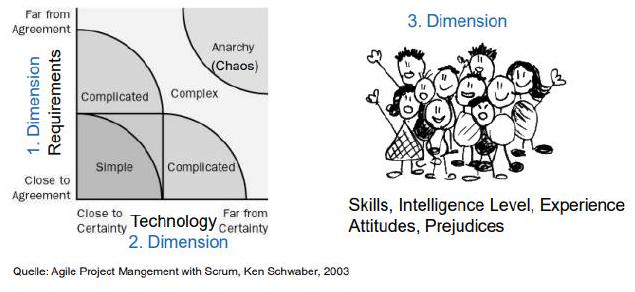
\includegraphics[width=\linewidth]{images/2024_12_29_0d1d7b5551ea1b4b41bdg-01}
\end{concept}

\begin{concept}{Modelle in der Softwareentwicklung} 
\begin{itemize}
    \item Software ist selbst ein Modell der Realität
    \item Anforderungsmodelle beschreiben das Problem
    \item Architektur-/Entwurfsmodelle beschreiben die Lösung
    \item Testmodelle beschreiben korrektes Verhalten
\end{itemize}
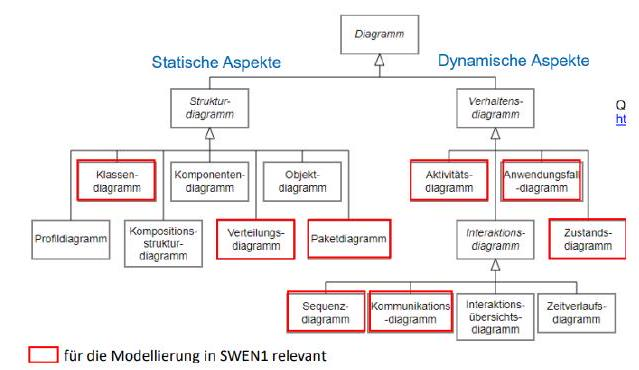
\includegraphics[width=\linewidth]{images/2024_12_29_0d1d7b5551ea1b4b41bdg-01(1)}
\end{concept}


\begin{formula}{Code and Fix}
\begin{itemize}
    \item Codierung und Korrektur im Wechsel
    \item Vorteile:
    \begin{itemize}
        \item Schnell und agil
        \item Einfach am Anfang
    \end{itemize}
    \item Nachteile:
    \begin{itemize}
        \item Schlecht planbar
        \item Schwer wartbar
        \item Änderungen aufwändig
    \end{itemize}
\end{itemize}
\end{formula}

\begin{formula}{Wasserfallmodell}
\begin{itemize}
    \item Sequentielle Phasen mit definierten Ergebnisdokumenten
    \item Vorteile:
    \begin{itemize}
        \item Gut planbar
        \item Klare Aufteilung in Phasen
        \item Definierte Meilensteine
    \end{itemize}
    \item Nachteile:
    \begin{itemize}
        \item Schlechtes Risikomanagement
        \item Spätes Kundenfeedback
        \item Unflexibel bei Änderungen
        \item Anforderungen nie vollständig zu Beginn bekannt
    \end{itemize}
\end{itemize}
\end{formula}

\begin{formula}{Iterativ-inkrementelle Modelle}
\begin{itemize}
    \item Schrittweise Entwicklung in geplanten Iterationen
    \item Vorteile:
    \begin{itemize}
        \item Flexibles Modell
        \item Gutes Risikomanagement
        \item Frühe Einsetzbarkeit
        \item Kontinuierliches Kundenfeedback
    \end{itemize}
    \item Nachteile:
    \begin{itemize}
        \item Planung upfront hat Grenzen
        \item Höherer Koordinationsaufwand
    \end{itemize}
    \item Basis für agile Entwicklung:
    \begin{itemize}
        \item Fokus auf funktionierender Software
        \item Kurze Iterationen
        \item Enge Kundeneinbindung
    \end{itemize}
\end{itemize}
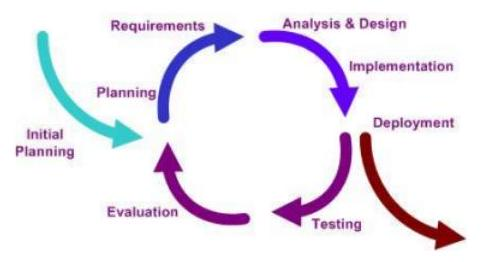
\includegraphics[width=0.8\linewidth]{images/2024_12_29_0d1d7b5551ea1b4b41bdg-02(1)}
\end{formula}


\begin{concept}{Charakteristiken iterativ-inkrementeller Prozesse}
\begin{itemize}
    \item Projekt-Abwicklung in Iterationen (Mini-Projekte)
    \item Inkrementelle Entwicklung (Stück für Stück)
    \item Risiko-getriebene Iterationsziele
    \item Reviews und Learnings nach jeder Iteration
    \item Demming-Cycle: Plan, Do, Check, Act
\end{itemize}
\end{concept}



\begin{KR}{Modellierungsumfang bestimmen}
Der benötigte Modellierungsumfang hängt ab von:
\begin{itemize}
    \item Komplexität der Problemstellung
    \item Anzahl beteiligter Stakeholder
    \item Kritikalität des Systems
    \item Domänenspezifische Anforderungen
    \item Analogie: Planung einer Hundehütte vs. Haus vs. Wolkenkratzer
\end{itemize}
\end{KR}

\begin{definition}{Unified Modeling Language (UML)}
Standardsprache für grafische Modellierung:
\begin{itemize}
    \item \textbf{Einsatz als:}
    \begin{itemize}
        \item Sketch: Informelle Kommunikation und Verständnis
        \item Blueprint: Detaillierte Design-Spezifikation
        \item Programming Language: Ausführbare Modellierung
    \end{itemize}
    \item \textbf{Vorteile:}
    \begin{itemize}
        \item Standardisierte Notation
        \item Verschiedene Abstraktionsebenen
        \item Unterstützung des gesamten Entwicklungszyklus
    \end{itemize}
\end{itemize}
%todo: add UML diagram types overview
\end{definition}

